\documentclass{article}
\usepackage{graphicx}
\usepackage[round]{natbib}
\usepackage{float}
\usepackage{fullpage}

\begin{document}
\title{Supplementary information for \texttt{phyx} (Phylogenetic tools for Unix)}

\author{Author, Co-Author, Stephen A. Smith\\\\
\normalsize{Department of Ecology \& Evolutionary Biology}\\
\normalsize{University of Michigan, Ann Arbor, MI 48109, USA}}
% address is not supported by article class?!? the above is hacky workaround
%\address{Department of Ecology \& Evolutionary Biology, University of Michigan, Ann Arbor, MI 48109, USA}
%\date{\today}
\date{} % no date
\maketitle

\section{Performance}
We briefly describe below the performance of \texttt{phyx} relative to other
existing tools.

\subsection{Sequence cleaning}
Cleaning sequences to ensure a certain level of matrix occupancy has become common place in many phylogenomic pipelines \citep{Dunn2013,YangSmith2014}. Here we compare two programs Gblocks \citep{Gblocks} and phyutility \citep{SmithDunn2008} to the sequence cleaning procedure of Phyx (pxclsq). The file sizes ranged from 10 sequences in the file (234Kb), to 100,000 sequences (2.3Gb) with all being 23,950 base pairs in length (see Supp. Figure 1). 
We found that Phyx outperformed both Gblocks and Phyutility in all dataset sizes and for the largest dataset Phyutility was not able to clean the dataset due to a memory allocation error. The test was conducted on a laptop  containing 4 processors and 16Gb of memory, with 14Gb of that memory being allocated for phyutility.

\begin{figure}[H]
    \centering
    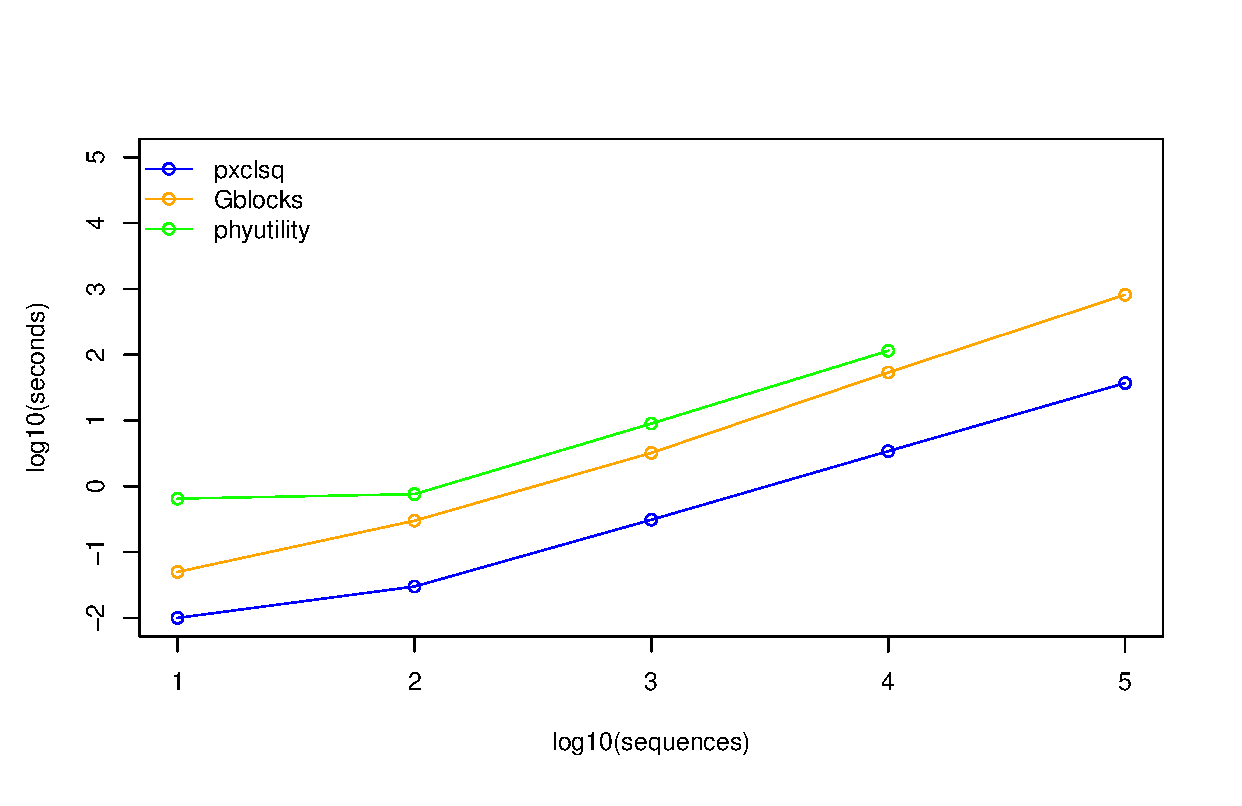
\includegraphics[width=3.0in]{clsq.eps}
    \caption{Comparison of alignment cleaning timings.}
    \label{cleaningfigure}
\label{fig:S1}
\end{figure}

\subsection{Conversion of proteins to codons}
Converting the alignment of proteins to their corresponding nucleotide file is useful in helping ensure accuracy in the nucleotide alignment. Here we tested files that were between 10 sequences of 801bp for the amino acid alignment(8.0kb) and 100,000 sequences of(77M). We found that Phyx was faster than PAL2NAL\cite{Suyama2006} under each condition. Also, Phyx does not require that the sequences be in the same order, thus reduce error and specifically avoiding aligning a nucleotide sequence with something other than its corresponding amino acid alignment.

\begin{figure}[h]
    \centering
    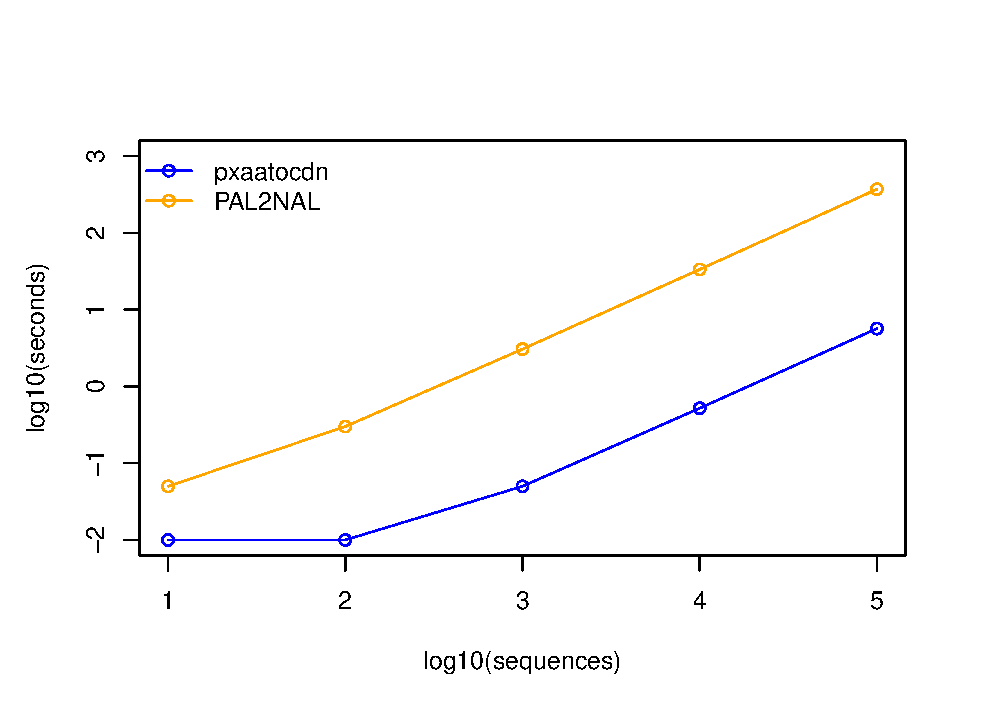
\includegraphics[width=3.0in]{aatocdn}
    \caption{Comparison of timings to convert protein alignemtns to
    their corresponding codon alignments.}
    \label{proteincodonfigure}
\label{fig:S2}
\end{figure}

\subsection{MCMC log concatenation and resampling}
MCMC log files from Bayesian phylogenetic analyses have become common phylogenetic objects. Such analyses are typically replicated (to ensure convergence of the MCMC chains) and run for many millions of generations (to achieve adequate effective sample sizes), resulting in several very large text files, each of which invariably involve a burnin phase (samples that are discarded before sumamrization). Prior to parameter summary, these log files are typically concatenated while removing the burnin phase and potentially resampling (thinning) the individual logs because of memory constraints. The \texttt{phyx} program \texttt{pxlog} carries out these operations on both tree and parameter logs. To assess the performance of \texttt{pxlog}, we compared it to two versions of \texttt{logcombiner} from the \texttt{BEAST} package \citep{DrummondRambaut2007,Bouckaert2014}. We ran phylogenetic in analyses in \texttt{BEAST} using the data from \cite{Magallon2015}, a data set which consists of 798 taxa. Five replicates MCMC analyses were performed, each running for 100 million generations and sampling trees every 5000 generations (for a total of 20000 trees sampled in each analysis). In preparation for tree summary, we discarded the first 25\% of samples, and further thinned the chains to every 10th sample (for a total of 1500 post-burnin samples per analysis).

\begin{figure}[!h]
    \centering
    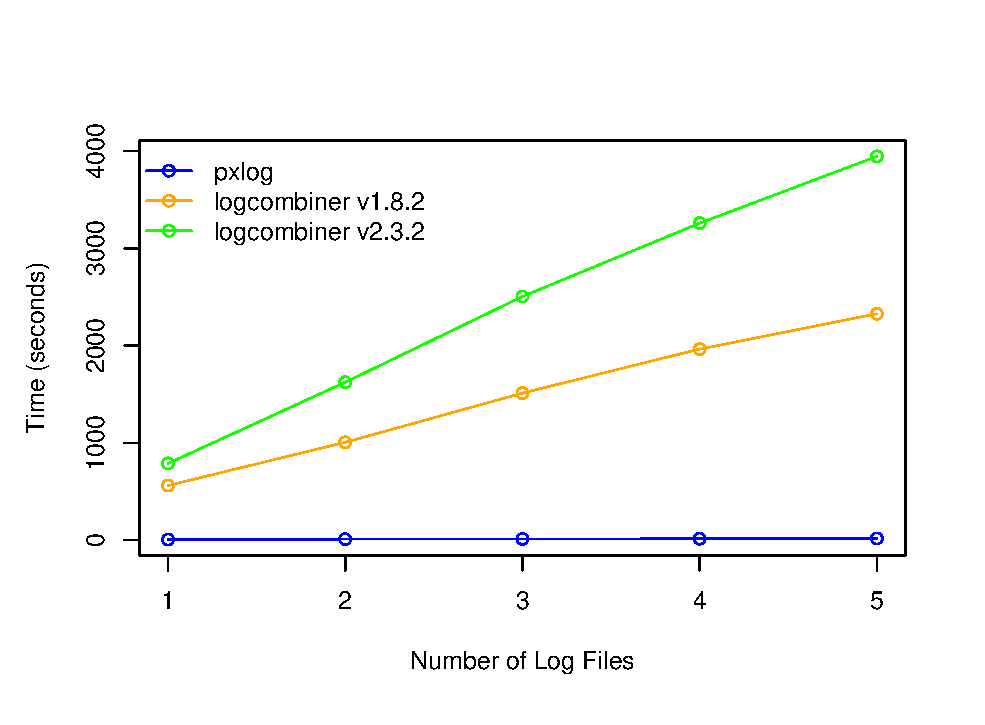
\includegraphics[width=3.0in]{log}
    \caption{Comparison of MCMC log manipulation timings. Each log file
    is 2.6 GB and contains 20000 trees.}
    \label{logfigure}
\label{fig:S3}
\end{figure}

The timings for the log manipulations by the various programs are displayed in Figure~\ref{fig:S3}. \texttt{pxlog} executed much faster than either version of \texttt{logcombiner} for any number of input files, taking only a few seconds compared to up to over an hour for the alternative tools. More revealing, however, was the memory usage of the various programs. \texttt{pxlog}, being stream-centric (and hence holding only a single tree in memory at any particular instant), consumed only 600 kb of RAM, despite the individual log files totalling 2.6 GB. \texttt{logcombiner} is a java-based tool to which we allocated 40 GB of RAM. \texttt{logcombiner} v1.8.2 was far more memory efficient than the newer version, consuming 2.4 GB of RAM for the full 5 file concatenation. \texttt{logcombiner} v2.3.2, on the other hand, consumed 32.6 GB of RAM while executing far more slowly.

\bibliographystyle{natbib} % want this one, but acting wonky
%\bibliographystyle{abbrv}
%\bibliographystyle{achemnat}
%\bibliographystyle{plainnat}
%\bibliographystyle{abbrv}
%\bibliographystyle{bioinformatics}
%
%\bibliographystyle{plain}
\bibliography{phyx}

\end{document}
